\chapter{L'OSINT}\label{chapter:OSINT}

L'open source intelligence (OSINT) è il processo di raccolta e analisi delle informazioni pubblicamente disponibili sulla rete, questi dati vengono poi utilizzati per valutare le minacce, prendere decisioni o rispondere a domande specifiche.

L'OSINT è generalmente definito come una qualsiasi azione di intelligence eseguita con l'utilizzo di informazioni pubblicamente consultabili (Open Source)\footnote{Giornali, riviste, TV, radio, report commerciali, social media, siti e forum}, che sia raccolto, ordinato e diffuso in modo tempestivo allo scopo di rispondere a requisiti specifici.

\begin{figure}[ht]
	\centering
	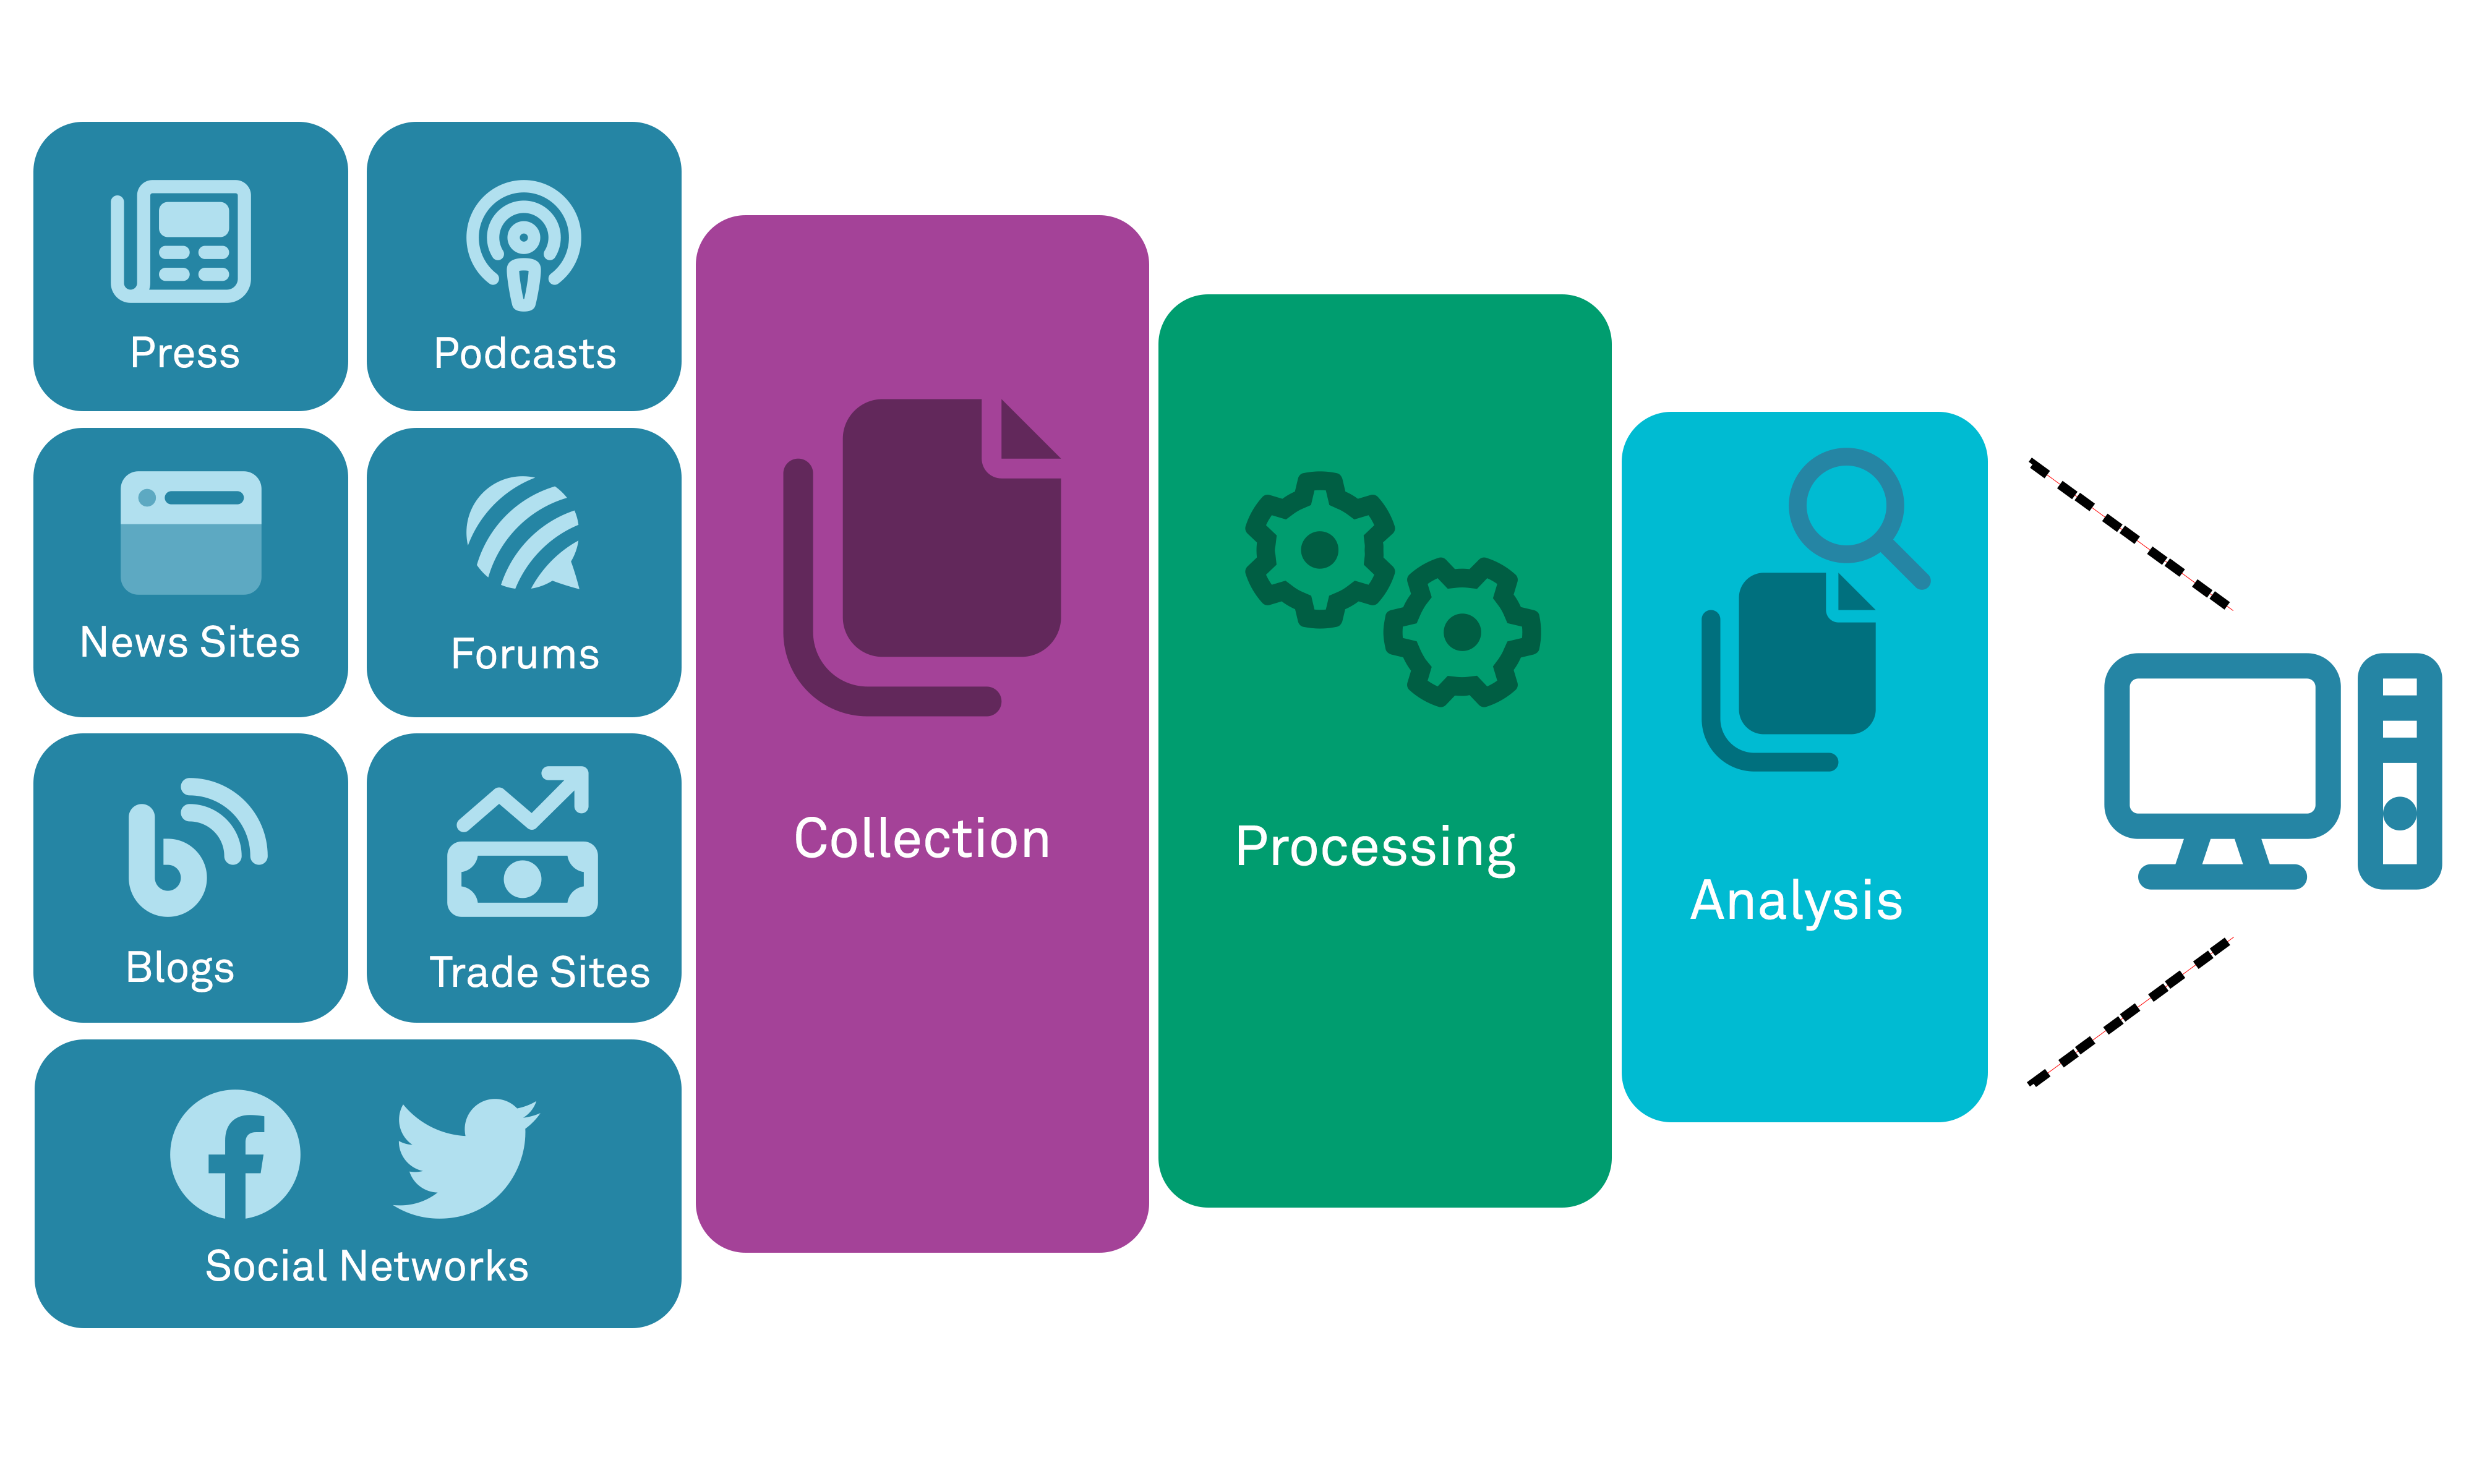
\includegraphics[width=0.8\textwidth]{Immagini/OSINT1.png}
	\caption{Processo generale di Open Source Intelligence}
	\label{fig:oneosint}
\end{figure}

\newpage
Questo tipo di dati assume connotazioni differenti a seconda di chi le utilizza, alcuni esempi:
\begin{itemize}
    \item Per la CIA, può significare informazioni ottenuto da trasmissioni di notizie straniere.
    \item Per un avvocato, può significare dati ottenuti da documenti governativi pubblicamente disponibili.
    \item E per la maggior parte delle persone, può significare la moltitudine di contenuti ottenibili da Internet.
\end{itemize}

Durante un'operazione di OSINT è consigliabile effettuare una serie di operazioni allo scopo di tutelarsi, partendo da un buon antivirus, dato che è fondamentale essere in possesso di un primo livello di protezione, nel caso in cui i dati consultati non fossero sicuri o eventuali informazioni scaricate contenessero dei virus.

Da notare che i normali antivirus sono in grado di proteggere il dispositivo, nel solo caso in cui il virus sia già conosciuto e categorizzato (non proteggono da ogni minaccia). 
Generalmente il programma preinstallato windows defender può essere sufficiente come barriera contro la maggior parte delle minacce conosciute.

\'E consigliabile inoltre che, se il sistema utilizzato sia Windows o Mac, sia predisposto un ulteriore livello di protezione da file dannosi, \textbf{Malware}, uno dei software più utilizzati a questo scopo è "Malwarebytes", software che permette la pulizia e la protezione del dispositivo da diversi tipi di minaccia malware.

Un altro consiglio per chiunque navighi "in profondità" sul web, è quello di utilizzare un web browser con più livelli di sicurezza e possibilità di plugin e estensioni, quali Firefox o Chrome.


\section{Definizione e Concetti Base dell'OSINT}\label{sec:cap_sec_osint1}

Come definito in precedenza l'Open Source Intelligence si riferisce alla raccolta, all'analisi e all'utilizzo di informazioni provenienti da fonti di informazione pubblicamente accessibili. 

I dati raccolti vengono elaborati e analizzati per estrarre da essi, informazioni significative. L'analisi delle informazioni dovrà includere l'eventuale correlazione di dati da fonti multiple, l'identificazione di schemi e tendenze, e la verifica dell'autenticità di queste ultime.

Esistono diversi strumenti e framework per eseguire attività di OSINT, come Maltego, The OSINT Framework, Shodan e molti altri.

Le principali aree di utilizzo delle tecniche elencate sono: 

\begin{itemize}
    \item Sicurezza Nazionale
    \item Cybersecurity
    \item Indagini Forensi e Criminali
    \item Protezione della Reputazione e dell'immagine
    \item Business Intelligence
    \item Stalking
\end{itemize}

Si ricorda che durante ogni operazione di raccolta dati è fondamentale rispettare la privacy, ed in particolare le normative sulla protezione dei dati (come il GDPR in Europa) e ogni altra legge locale e internazionale.

\'E indispensabile poi sottolineare che non tutte le informazioni disponibili pubblicamente sono accurate o affidabili; è necessario infatti un processo rigoroso di verifica e validazione. Il volume dei Dati, potrebbe presentarsi come un'ulteriore sfida, considerato che la gestione di un'enorme quantità di dati provenienti da diverse fonti può essere complessa e necessità di essere eseguita in modo rigoroso, con l'analisi del contesto\footnote{Comprendere il contesto delle informazioni raccolte è fondamentale per evitare interpretazioni errate.}.

Con l'evoluzione di Internet e la crescita delle piattaforme digitali, l'OSINT continua ad espandersi, sfruttando anche l'intelligenza artificiale e il machine learning per migliorare l'analisi dei dati e la previsione delle minacce.

\begin{figure}[ht]
	\centering
	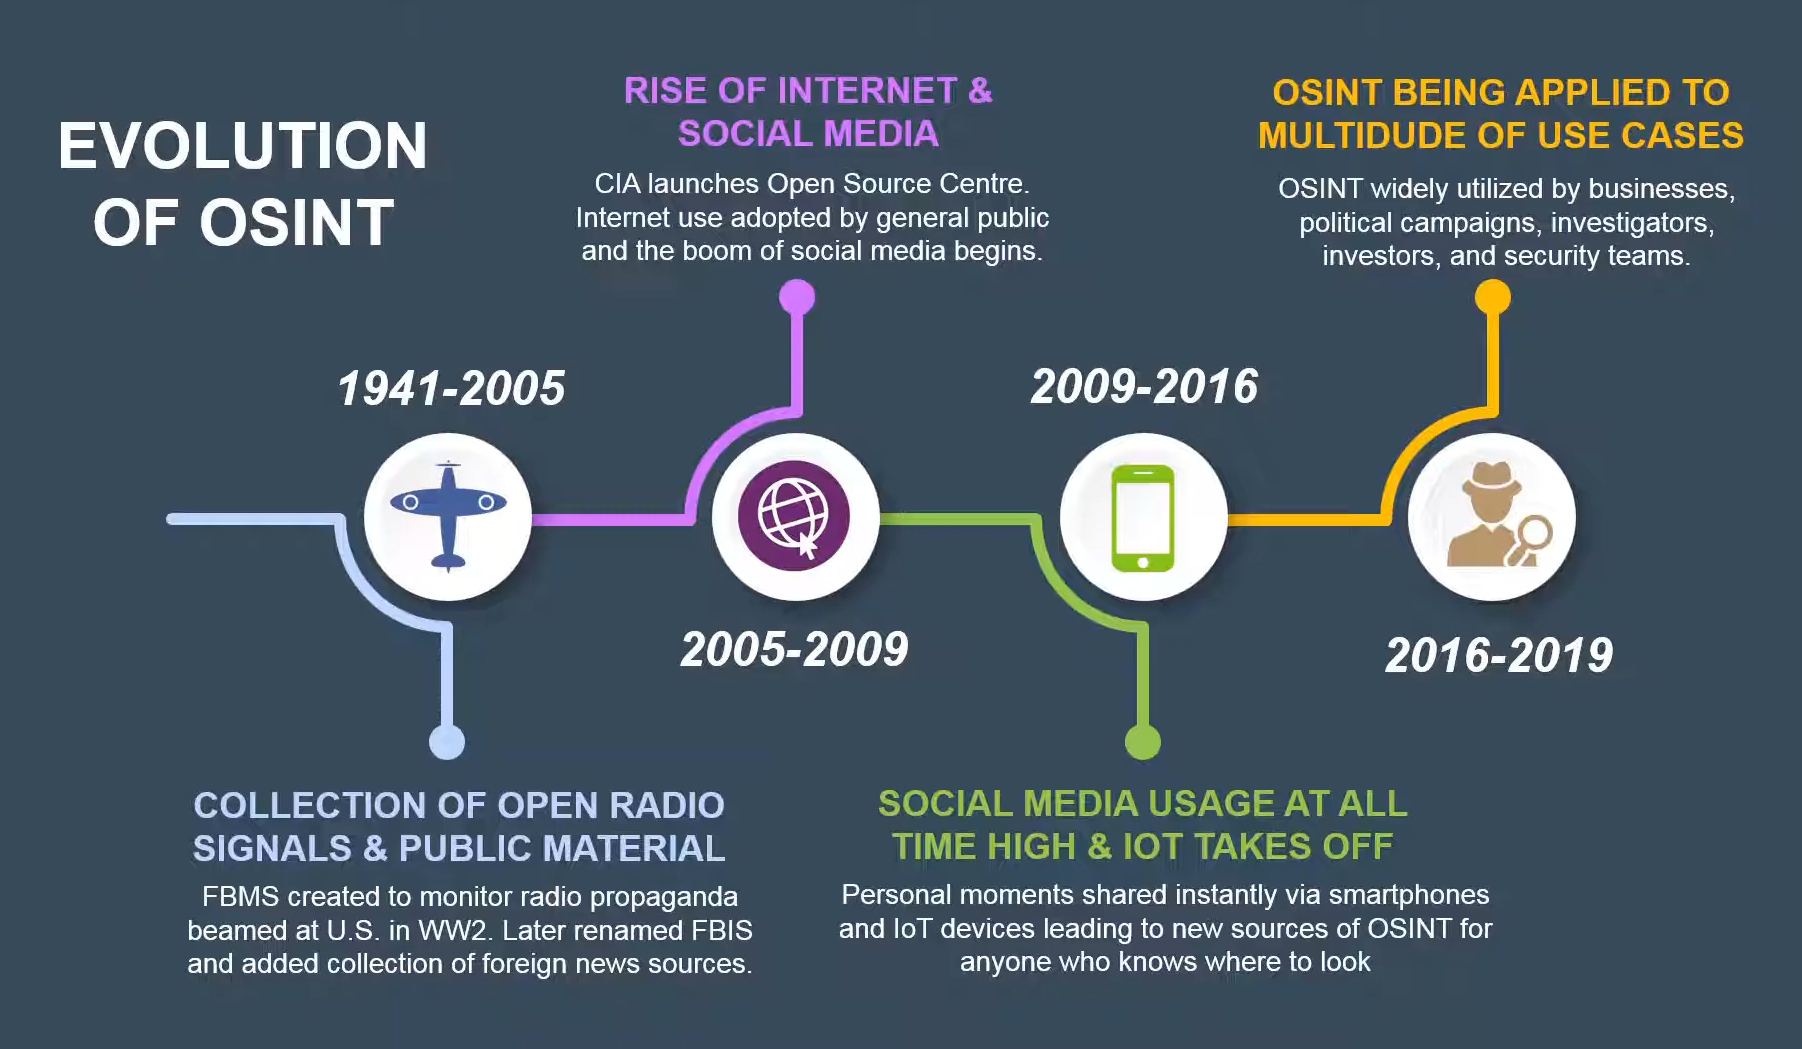
\includegraphics[width=0.8\textwidth]{Immagini/OSINT2.png}
	\caption{Attori OSINT}
	\label{fig:twoosint}
\end{figure}

\newpage
La Storia dell'OSINT è riconducibile agli albori della Seconda guerra mondiale, con l'istituzione del BBC Monitoring Service nel Regno Unito, 1939, e del Foreign Broadcast Monitoring Service (FBMS) negli Stati Uniti, 1941. 
Sebbene questi due servizi siano stati istituiti in risposta all'avvento della radiofonia e siano certamente esempi dei primi sforzi strutturali per raccogliere e sfruttare informazioni pubblicamente disponibili, è certo che l'OSINT abbia una storia istituzionale molto più lunga.

L'Open Source Intelligence ha ricevuto un'attenzione crescente negli ultimi decenni, in particolare con l'avvento dell'era dell'informazione e con l'ascesa di internet, grazie inoltre ai domini digitali per la produzione e l'archiviazione dei dati è avvenuto un cambiamento radicale per tutte le comunità d'Intelligence.

Il primo utilizzo pubblico della frase "open-source intelligence" e dell'acronimo "OSINT" nella letteratura sugli studi sull'intelligence risale ad un articolo del 1990 di Robert Steele \footnote{Robert David Steele (1952 – 2021) American case officer for the Central Intelligence Agency, co-founder of the United States Marine Corps Intelligence Activity}


\newpage
Sebbene la raccolta e lo sfruttamento di dati da fonti pubblicamente accessibili non avesse guadagnato importanza fino a questo momento, l'utilità dei dati da fonti pubbliche risale a molto tempo prima.
Per esempio l'uso pratico delle fonti aperte durante la Seconda Guerra Mondiale, documentate da diverse pubblicazioni risalenti al 1946, da William Donovan. Tuttavia, ci volle fino agli anni '90 prima che l'acronimo "OSINT" iniziasse a essere utilizzato e ci vollero altri due decenni prima che quell'uso diventasse diffuso nella letteratura sugli studi sull'intelligence.

Viene sostenuto da diversi autori che ciò che oggi chiamiamo OSINT, esisteva ed era già presente millenni fa, questo dato che dai legionari romani, ai vichinghi, ai mercanti della Via della Seta, venivano conservate e ricercate informazioni, osservando il mondo circostante, allo scopo di poter poi comprendere e diffondere le conoscenze ad altri. Da notare però che "non è stato un sforzo metodico fino a quando gli Stati Uniti non hanno fatto da pionieri nell'istituzionalizzazione e professionalizzazione di una capacità autonoma di monitoraggio dei media stranieri, con l'istituzione del \textbf{Foreign Broadcast Monitoring Service}"\cite{osint2}.

\section{Importanza e Applicazioni dell'OSINT}\label{sec:cap_sec_osint2}

I risultati possono essere utilizzati per individuare fughe non autorizzate di dati proprietari o sensibili, valutare la sicurezza delle informazioni e identificare vulnerabilità come software senza patch, configurazioni errate o porte aperte. Le organizzazioni possono anche condurre test di penetrazione dei propri sistemi e reti utilizzando gli stessi dati OSINT accessibili al pubblico da criminali informatici e hacker.

Spesso, le informazioni raccolte durante una valutazione OSINT vengono combinate con dati non pubblici per creare un report di threat intelligence più completo. Gli aggiornamenti di OSINT sulla cybersecurity possono aiutare le organizzazioni a mitigare il rischio di violazioni dei dati, ransomware, malware e altri attacchi informatici.\cite{osint1}

L'Open Source Intelligence può essere sia attiva che passiva.
Quello passivo comprende la raccolta e l'analisi dei dati, senza interagire direttamente con essi o con la loro sorgente. Per esempio un'intelligence di questo tipo può essere la ricerca e la raccolta di dati online da siti, social media e database pubblici, immagini satellitari e mappe.
Rientra in questa tipologia anche la consultazione di documenti pubblici, report e articoli.

Quello attivo riguarda invece tutte quelle tecniche o operazioni che necessitano di un'interazione con la fonte, con gruppi o con utenti finali, i quali andranno a fornire i dati richiesti. Alcuni esempi sono, prendere parte ad un forum online, ad una discussion board o a diverse community presenti sui social riguardo ad uno specifico argomento. 

Condurre colloqui, interviste o sondaggi e raccogliere informazioni da singoli o esperti di un determinato settore. Fanno parte di questa tipologia di dati, quelli raccolti prendendo parte a conferenze, osservando ed interagendo con il pubblico presente.

\begin{figure}[ht]
	\centering
	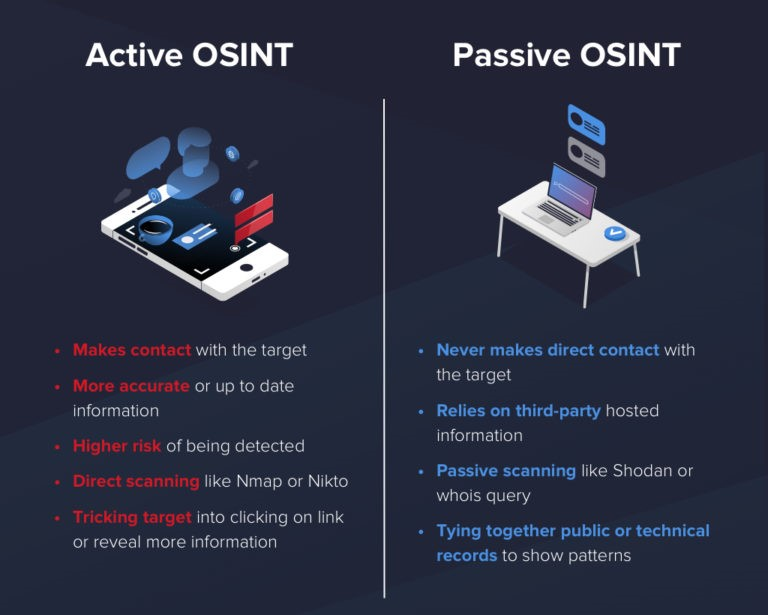
\includegraphics[width=0.8\textwidth]{Immagini/OSINT3.jpeg}
	\caption{Active and Passive Open Source Intelligence}
	\label{fig:threeosint}
\end{figure}

\newpage
\section{Tecniche e Strumenti di Raccolta Dati}\label{sec:cap_sec_osint3}

Secondo Neotas\footnote{Azienda specializzata nell'Open Source Intelligence, analisi dati, Intelligenza Artificiale (AI), che mette a disposizione diversi servizi all'avanguardia, background checks e Risk assessment, allo scopo di aiutare diverse aziende a prendere decisioni informate e a gestire i rischi in modo efficace.} e IBM \footnote{"Big Blue", è un'azienda statunitense del settore informatico, tra le più importanti al mondo. Produce e commercializza hardware, software e servizi informatici, offrendo infrastrutture, servizi di hosting, cloud, intelligenza artificiale, computazione quantistica e consulenza} esistono diverse tecniche e strumenti per condurre attività di intelligence:

	\begin{enumerate} 
	\item \textbf{Per il Web Data Scraping: }
		\begin{enumerate}
			\item Advanced Scraping Frameworks: Strumenti come Scrapy (Python) e Apify mettono a disposizione capacità di scaping \footnote{tecnica informatica di estrazione di dati da un sito web} molto avanzate, incluso il trattamento di contenuti renderizzati tramite JavaScript, rotating proxies e scalando le operazioni di scraping su più macchine. 
			\item Headless Browsing: Sono browser senza interfaccia come Puppeteer (Node.js) e Selenium, i quali permettono uno scraping dinamico e AJAX (abbreviazione di Asynchronous JavaScript and XML) che permettono al programma di interagire con la pagina web, come fosse un'utente reale.
            \item Estrazione e Parsing dei dati: Utilizzo di tecniche avanzate con l'impiego di modelli di machine learning per un'estrazione intelligente, come il naming entity recognition (NER) e l'optical character recognition (OCR) per l'estrazione di testo da immagini e PDFs.
		\end{enumerate}

    \item \textbf{Social Media Intelligence (SOCMINT):}
        \begin{enumerate}
            \item Tecniche avanzate di monitoring dei Social Media: Strumenti quali Brandwatch, Crimson Hexagon, and Synthesio permettono un monitoring globale su più social media, fornendo analisi, riconoscimento di trend e utenti di rilievo.
            \item Analisi dei Network: Strumenti per l'analisi della rete come Gephi and NodeXL possono essere utilizzate per visualizzare e analizzare social networks, identificare influencers, scoprire communities, e scoprire legami nascosti tra utenti e gruppi.
            \item Natural Language Processing (NLP): Le NLP sono tecniche, quali la modellazione dei dati, l'analisi dei sentimenti e il riconoscimento di entità possono essere applicati ai social media, per poter estrarre informazioni preziose, scoprire nuove tendenze e identificare potenziali rischi e minacce.
        \end{enumerate}

    \item \textbf{Dark Web Monitoring:}
        \begin{enumerate}
            \item Crawlers e Scrapers automatici: Strumenti che come la libreria del progetto Tor e Scrapy-Splash Permettono il crawling e lo scraping automatico dei contenuti presenti sul dark web, permettendo la raccolta di dati su vasta scala.
            \item Ambienti virtuali e Sandboxing\footnote{Ambiente sicuro e isolato su una rete, il quale imita gli ambienti operativi reali/finali}: Macchine virtuali, containers, e sandboxing sono spesso utilizzate per accedere e analizzare in modo sicuro, materiale proveniente dal dark web, isolando il sistema da potenziali minacce e mantenendo il sistema in sicurezza.
            \item Monitoring di transazioni di Cryptovalute: I tool per l'analisi del Blockchain come Chainalysis and Elliptic permettono di monitorare e tracciare le transazioni che avvengono con le cryptovalute, potenzialmente scoprire transazioni illecite e attività sul dark web.
        \end{enumerate}
        \setcounter{TMPenumnbr}{\value{enumi}}
\end{enumerate}

\begin{figure}[ht]
	\centering
	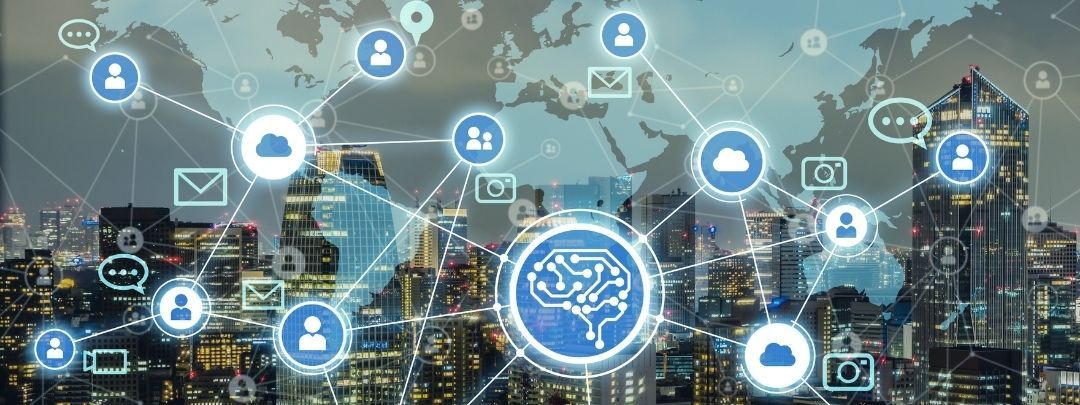
\includegraphics[width=1\textwidth]{Immagini/OSINT4.jpeg}
	\caption{Social e Data Monitoring}
	\label{fig:fourosint}
\end{figure}

\newpage

\begin{enumerate}
\setcounter{enumi}{\value{TMPenumnbr}}
    \item \textbf{Intelligence Geospaziale (GEOINT):}
        \begin{enumerate}
            \item Telerilevamento e Analisi di Immagini Satellitari: Tecniche più avanzate comprendono l'uso di dati di telerilevamento provenienti da fonti quali, Landset, Sentinel e fornitori commerciali uniti ad algoritmi di machine learning e rilevamento di oggetti, cambiamenti e pattern recognition.
            \item Modellazione e visualizzazione 3D: Tools come ArcGIS Pro e ENVI possono essere utilizzati per creare modelli 3D di aree geografiche, per l'analisi dei dettagli di un territorio, per le infrastrutture e per diverse attività.
            \item Integrazione dei dati geospaziali: L'integrazione di vari dati geospaziali, come immagini satellitari, fotografie aeree e dati GIS, possono fornire numerosi dati per un'area di interesse.
        \end{enumerate}

    \item \textbf{Analisi del Traffico di Rete:}
        \begin{enumerate}
            \item Deep Packet Inspection (DPI): Le tecniche DPI comportano l'ispezione dei dati contenuti nei pacchetti di rete, consentendo un'analisi dettagliata del traffico di rete, la rilevazione di attività sospette o l'estrazione del traffico crittografato.
            \item Network Behavior Analysis: Strumenti quali Zeek (conosciuto anche come Bro) e Suricata possono essere utilizzate per l'analisi dei pattern del traffico di rete, individuare anomalie e scoprire potenziali minacce.
            \item Network Flow Analysis: Strumenti di analisi del flusso di rete come SiLK e Argus possono essere utilizzati per l'analisi dei flussi di rete, fornendo informazioni sui pattern di comunicazione, sull'utilizzo della banda di rete e potenziali incidenti di sicurezza.
        \end{enumerate}

    \item \textbf{Informatica Forense:}
        \begin{enumerate}
            \item Memory Forensics: Strumenti quali Volatility and Rekall possono essere utilizzati per analizzare ed estrarre i dati da system memory dump di sistemi, consentendo il recupero di dati crittografati, file eliminati e numerose risorse forensi.
            \item Disk and File System Forensics: Sono tecniche avanzate, che prevedono l'utilizzo di strumenti come The Sleuth Kit, EnCase, e FTK per eseguire un'analisi approfondita delle immagini del disco e del file system, per recuperare dati cancellati e per l'analisi di metadati e prove digitali.
            \item Malware Analysis: Strumenti di sandboxing come Cuckoo Sandbox e Joe Sandbox possono essere utilizzati per l'analisi dinamica di Malware, consentendo l'esecuzione controllata e il monitoraggio di codice potenzialmente dannoso, per poterne capire il funzionamento.
        \end{enumerate}

    \item \textbf{Machine Learning e Intelligenza Artificiale:}
        \begin{enumerate}
            \item Natural Language Processing (NLP): Le NLP sono tecniche, come detto, quali la modellazione dei dati, l'analisi dei sentimenti e il riconoscimento di entità possono essere applicati ai social media, possono essere utilizzate anche su grandi database, allo scopo di estrarre informazioni.
            \item Computer Vision e Image Recognition: I modelli del Machine learning possono essere allenati per l'analisi e la classificazione di immagini, oggetti, e per l'identificazione di pattern.
            \item Predictive Analytics e Rilevamento anomalie: Tecniche quali il clustering, e il rilevamento delle anomalie possono essere utilizzate per l'identificazione di pattern, prevedere eventi futuri e rilevare minacce all'interno di grandi insiemi di dati.

            
            \end{enumerate}

\begin{figure}[ht]
	\centering
	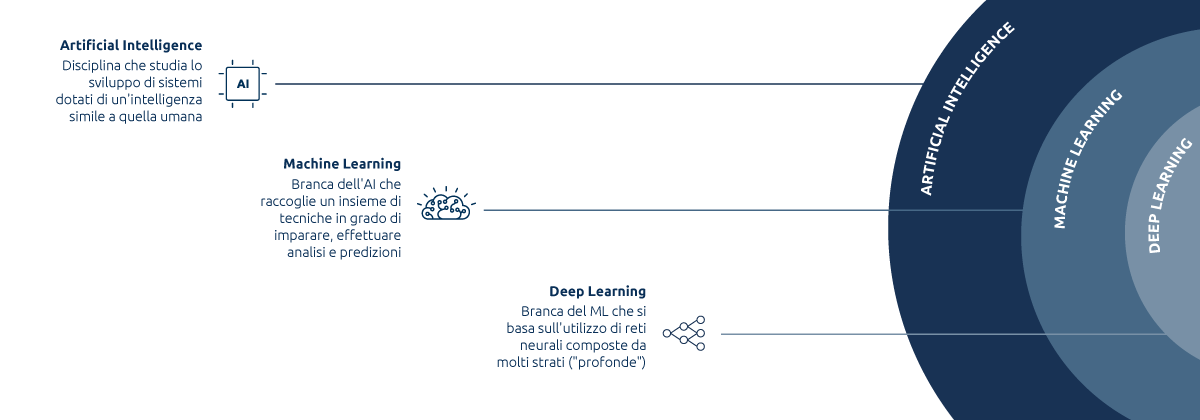
\includegraphics[width=1.2\textwidth]{Immagini/OSINT5.png}
	\caption{Intelligenza Artificiale e Machine Learning}
	\label{fig:fiveosint}
\end{figure}

\newpage

    \item \textbf{Data Visualisation e Link Analysis:}
        \begin{enumerate}
            \item Visualizzazione interattiva dei Dati: Strumenti quali Tableau, Power BI, e D3.js permettono la creazione di visualizzazioni interattive e dinamiche, consentendo agli analisti di esplorare e presentare i dati in modo intuitivo e leggibile.
            \item Analisi di link e Visualizzazione Grafici: Strumenti come Neo4j, Gephi, e Palantir permettono l'analisi dei collegamenti e la visualizzazione di grafici, aiutando gli analisti ad individuare in modo più rapido e preciso, connessioni nascoste e comprendere relazioni complesse tra i dati.
            \item Visualizzazione dei dati Geospaziali: Software GIS\footnote{Un sistema informativo in grado di associare dei dati alla loro posizione geografica sulla superficie terrestre e di elaborarli per estrarne informazioni} come ArcGIS e QGIS possono essere usati per visualizzare e analizzare dati geospaziali, consentendo la creazione di mappe interattive, unendo diversi dati e diverse risorse, per l'identificazione di trend e pattern.
        \end{enumerate}
	\end{enumerate}


Queste tecniche avanzate di OSINT spesso richiedono competenze particolari, oltre a una profonda comprensione dell'analisi dei dati e della programmazione. Sono tipicamente impiegate da agenzie di intelligence, forze dell'ordine, professionisti della sicurezza informatica e ricercatori per raccogliere informazioni, scoprire minacce e ottenere una visione completa di situazioni o fenomeni complessi.


Al giorno d'oggi, quasi tutti possono partecipare alla raccolta di open source intelligence, alcune delle fonti pubbliche da cui chi utilizza l'OSINT può raccogliere dati includono: Motori di ricerca internet come Google, DuckDuckGo, Yahoo, Bing e Yandex, mezzi di informazione cartacei e online, come giornali, riviste e siti di notizie, social network quali Facebook, Twitter(X), Instagram e LinkedIn, forum online e blog, il dark web, un'area crittografata di internet non indicizzata dai motori di ricerca, elenchi online di numeri di telefono, indirizzi e-mail e indirizzi fisici, registri pubblici di nascite, decessi, atti giudiziari e documenti aziendali, documenti governativi come trascrizioni delle riunioni, bilanci, discorsi e comunicati stampa emessi dai governi locali, statali e federali/nazionali, ricerche accademiche, inclusi documenti, tesi e riviste, dati tecnici quali indirizzi IP, API, porte aperte e metadati delle pagine web.
\newpage

L'OSINT Framework è un insieme completo di processi, tecniche e strumenti progettati per facilitare la raccolta, l'elaborazione, l'analisi e la diffusione di informazioni ottenute da fonti open e pubbliche. Comprende numerose fonti di dati, tra cui siti web, social media, registri pubblici, notizie, pubblicazioni accademiche e altri materiali.



\section{Limiti e Sfide dell'OSINT}\label{sec:cap_sec_osint5}

Le considerazioni etiche sono fondamentali nel campo della raccolta di OSINT. \'E fondamentale aderire a standard legali come il Regolamento Generale sulla Protezione dei Dati (GDPR) e garantire la raccolta etica dei dati. Rispettare i termini di servizio, mantenere la trasparenza e salvaguardare la privacy individuale, che devono essere sempre rispettati durante tutto il processo di OSINT.

Durante l'uso di una qualsiasi tecniche di OSINT è fondamentale tener conto di alcuni ostacoli:

\begin{enumerate}
    \item Information overload:  L'enorme volume di dati pubblicamente disponibili, in quanto queste informazioni, provengono da varie fonti online e può risultare una mole travolgente di informazioni, e può rendendo difficile identificare informazioni rilevanti e affidabili.
    \item Verifying source credibility: In quanto è indispensabile valutare la credibilità e l'affidabilità delle fonti di informazioni raccolte, poiché le fonti aperte possono contenere inesattezze, bias o disinformazione.
    \item Legal and ethical constraints: I professionisti dell'OSINT devono navigare tra i confini legali ed etici, rispettare la privacy e i diritti di proprietà intellettuale, e aderire alle normative e politiche pertinenti.
    \item Rapidly evolving data landscapes: Siccome l'evoluzione costante delle piattaforme online, dei formati dei dati e delle tecnologie richiede un adattamento continuo e lo sviluppo di nuove tecniche e strumenti OSINT.
\end{enumerate}

A questo punto una domanda sorge spontanea, l'OSINT è legale?

L'OSINT è generalmente considerato legale in quanto implica la raccolta e l'analisi di informazioni provenienti da fonti pubblicamente disponibili. Tuttavia, è fondamentale seguire le linee guida, per quanto concerne la legalità e l'eticità, rispettare i diritti di proprietà intellettuale e evitare qualsiasi accesso non autorizzato o pratiche di raccolta dati illegali. 
Le considerazioni etiche, come la protezione della privacy e la trasparenza, sono anch'esse essenziali quando si conducono attività di OSINT.

I tre pilastri dell'OSINT sono:
\begin{enumerate}[I]
    \item Conformità Legale ed Etica: Garantire che le attività di OSINT siano conformi alle leggi, regolamenti e standard etici, rispettando la privacy e i diritti di proprietà intellettuale.
    \item Trasparenza: Promuovere la trasparenza nei processi di OSINT, nelle metodologie e nell'uso dei dati pubblicamente disponibili, favorendo la fiducia e la responsabilità.
    \item Adattabilità: Adattarsi ai dati in continua evoluzione, incorporando nuovi strumenti, tecniche e metodologie per rimanere aggiornati ed efficaci di fronte ai progressi tecnologici e ai cambiamenti negli ambienti.
\end{enumerate}


L'Open Source Intelligence ha però un lato oscuro, il quale si riferisce al potenziale uso improprio delle tecniche e degli strumenti di intelligence da fonti aperte per scopi illegali, non etici o dannosi.

Questi usi illeciti possono essere, la raccolta di informazioni per attacchi informatici, condurre sorveglianza non autorizzata o violare i diritti alla privacy, spionaggio aziendale, il furto di segreti commerciali, violazione di proprietà intellettuale, diffondere disinformazione, propaganda, fake news ed infine impegnarsi in pratiche di raccolta dati non etiche o illegali, come lo scraping senza autorizzazione o la violazione dei termini di servizio.

\let\cleardoublepage\clearpage